\documentclass[10pt,journal,compsoc]{IEEEtran}

\usepackage{verbatim}
\usepackage{url}
\usepackage{graphicx}

\usepackage{xspace}
\newcommand{\FC}       {Freechains\xspace}
\newcommand{\reps}     {\emph{reps}\xspace}
\newcommand{\onerep}   {\emph{1~rep}\xspace}
\newcommand{\nreps}[1] {\emph{#1~reps\xspace}}
\newcommand{\code}[1]  {\texttt{\footnotesize{#1}}}
\newcommand{\Xon} {$1{\rightarrow}N$\xspace}
\newcommand{\Xno} {$1{\leftarrow}N$\xspace}
\newcommand{\Xnn} {$N{\leftrightarrow}N$\xspace}
\newcommand{\Xoo} {$1{\leftrightarrow}1$\xspace}
\newcommand{\Xo}  {$1{\hookleftarrow}$\xspace}

\renewcommand{\theenumi}{\alph{enumi}}

\hyphenation{off-line}

\begin{document}

\title{
    Symmetric Peer-to-Peer Applications
}

\author{
    Francisco Sant'Anna~\IEEEmembership{Department of Computer Science, Rio de Janeiro State University}
}

\IEEEtitleabstractindextext{%
\begin{abstract}
In multi-node collaborative applications, such as shared online documents,
users can interact remotely and yet share the exact same experience as if they
were in a single machine.
%
In this work, we propose a middleware for \emph{symmetric peer-to-peer
applications} in which decentralized instances can broadcast asynchronous
events and yet conform to identical behavior.
%
Nodes are allowed to join and leave the network at any time.
Application developers must adhere to a restricted API, which is
deterministic, stateless, and only supports pre-allocated memory.
%
The middleware is responsible for synchronizing the events in a global shared
timeline across the network.
Based on memory snapshots and deterministic simulation, a ``time machine'' can
rollback conflicting peers to resynchronize their state.
%
TODO: application, results
\end{abstract}

\begin{IEEEkeywords}
collaboration, determinism, peer-to-peer, time machine
\end{IEEEkeywords}}

\maketitle

% TOTAL: 12 pages

\section{Introduction}
\label{sec.introduction}

\IEEEPARstart{C}{ollaborative} networked applications allow multiple users to
interact remotely and yet share the same experience in real time.
Examples of these \emph{symmetric distributed applications}~\cite{gals} are
shared documents, watch parties, and multi-player games.
%
In order to reproduce the exact behavior in multiple devices, the application
must be able to synchronize time and execution across the network.
In addition, since users can interact asynchronously with the application,
event occurrences must somehow be synchronized back across devices.

A common approach towards symmetric applications is to introduce a middleware
to orchestrate events and time in the network~\cite{gals,croquet}.
This way, applications developers can rely on middleware primitives to trigger
events, which are intercepted and synchronized in a global shared timeline
across the network.
Developers must also restrict themselves to deterministic and stateless calls
only, such that execution can be equally reproduced in all nodes according to
the shared timeline.
However, current solutions depend on a central server to interconnect network
nodes and determine the shared timeline.

In this work, we propose \emph{symmetric peer-to-peer applications}, which
do not rely on central servers for coordination.
Nodes in the application form a dynamic graph network and communicate only
with direct neighbours.
Events are flooded in the graph and are triggered locally with a small delay
to consider the network latency.
To deal with events received out of order or too late, a distributed time
machine can rollback peers to a previous state and reapply events in order and
in time.

TODO: application, results

In Section~\ref{sec.related}, we revisit existing solutions for symmetric
distributed applications.
In Section~\ref{sec.tml}, we detail our proposed middleware.
In Section~\ref{sec.app}, ...
In Section~\ref{sec.eval}, ...
In Section~\ref{sec.conclusion}, ...

- assumptions
    - correct (non-malicious) nodes

- local first
- p2p
- less restrictive (compared to CRDTs)
- semantic events
    - limitation b/c of rollbacks
    - features b/c of network traffic

\section{Related Work}
\label{sec.related}

% docs.google.com/spreadsheets/d/1CpMmEgabJq2XQeTDW_BNCV4JWrcMlELuaEjDtw7kwg0/
\begin{figure}[t]
  \centering
  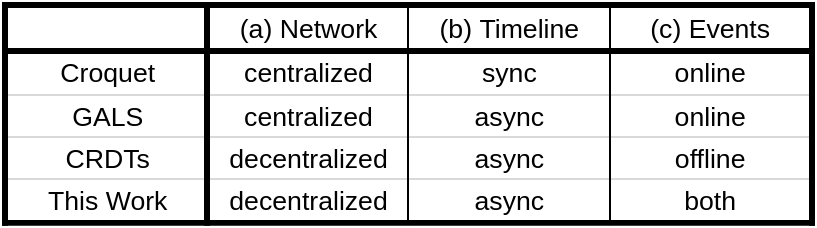
\includegraphics[width=\linewidth]{table}
  \caption{
    \label{fig.table}
  }
\end{figure}

\begin{figure*}[t]
  \centering
  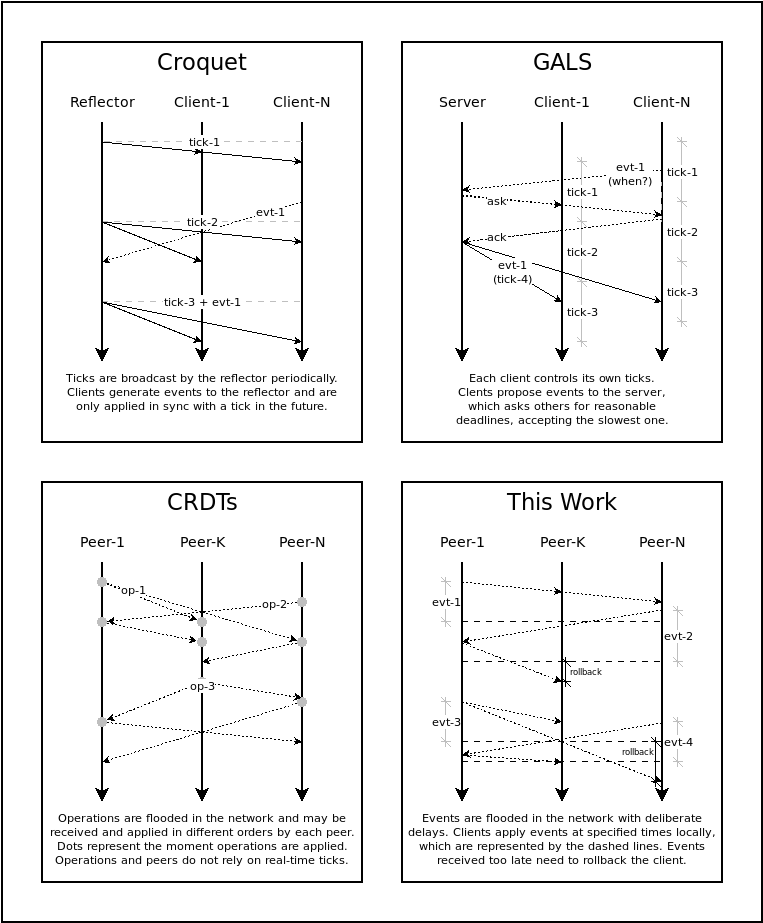
\includegraphics[width=\linewidth]{algos}
  \caption{
    \label{fig.algos}
    Four approaches to symmetric distributed applications: Croquet, GALS,
    CRDTs, and this work.
    The vertical arrows in parallel represent the timelines in nodes in the
    network.
    The arrows crossing nodes represent communication between them.
  }
\end{figure*}

In this section, we revisit existing solutions for symmetric distributed
applications.
We focus on (i) how the network is organized, (ii) how global time is
determined, and (iii) how events are propagated and applied.
Figure~\ref{fig.table} compares selected works regarding these aspects.

Croquet%
\footnote{Croquet.io: https://croquet.io/}~\cite{croquet} guarantees
bit-identical real-time behavior for every user in a collaborative
distributed environment.
%
As detailed in Figure~\ref{fig.algos}, a centralized \emph{reflector} issues
periodic ticks, such that all nodes in the network advance together according
to a synchronized global shared clock.
If an user generates an event, it is delayed and sent back to the reflector,
which broadcasts the event in the next tick, which all nodes apply in sync
(including the originating node).
%
Croquet takes periodic snapshots of the whole application state in order to
support late joins to a running session.
The new node just needs to restore the latest snapshot and simulate the
remaining events to reach the current running state.
%
As indicated in Figure~\ref{fig.table}, Croquet relies on a centralized
network, in which nodes advance in sync, and in which event outcomes depend
on the central server to be online.

GALS~\cite{gals} shares the same goals with Croquet, but with some tradeoffs,
mostly favoring clients with slow connections.
As detailed in Figure~\ref{fig.algos}, instead of advancing ticks in sync with
the server, clients have their own local clocks.
Also, event generation is delayed dynamically according to the slowest client.
%
On the one hand, ticks do not generate any traffic and clients have smooth
frame transitions, even those with poor connections.
On the other hand, event generation requires two round trips to the server and
clients may experience occasional freezes.
The syncing protocol also requires bookkeeping to deal with clock drifts and
client disconnections~\cite{gals}.
%
As indicated in Figure~\ref{fig.table}, GALS relies on a centralized
network, in which nodes advance independently, and in which event outcomes
depend on the central server to be online.

In both solutions, the network advances together as a whole in real time, with
a total order among events, which is determined by a central server that must
be permanently online.
All clients compute the events in sequence, respecting their timestamps, and
using only deterministic and stateless calls.
This way, it is guaranteed that all clients reach the same state, also going
through bit-identical steps.

An antagonistic approach to deterministic reactions to events is to model the
application with conflict-free replicated data types (CRDTs)~\cite{crdts}.
CRDTs are designed in such a way that all operations are commutative, so that
the order in which they are applied does not affect the final outcome.
%
As detailed in Figure~\ref{fig.algos}, peers can communicate operations
directly to each other with no central authority.
Also, since operations need not to be ordered, they can be applied at the
very first moment they are generated or received, even if the peers are
offline.
%
Since operations must be commutative, it is not possible to timestamp them
in a global shared clock.
Hence, there is no notion of a timeline in which peers go through
bit-identical steps, but they do eventually reach the same state.
%
On the one hand, the main advantage of CRDTs is the support for local-first
software~\cite{local}, since they can work offline in the same way as online.
On the other hand, they provide very restrictive APIs (the CRDTs themselves),
and do not support real-time consensus among peers.
%
As indicated in Figure~\ref{fig.table}, CRDTs work on decentralized networks,
in which peers advance independently, and in which operations can be applied
immediately, even while offline.
%
Automerge along with its accompanying Hypermerge peer-to-peer infrastructure
is an example of an implementation of decentralized
CRDTs~\cite{p2p.automerge,p2p.pushpin}.

In this work, as indicated in Figure~\ref{fig.table}, our goal is to support
peer-to-peer real-time symmetric execution, while still tolerating offline and
out-of-order event generation.
%
As detailed in Figure~\ref{fig.algos}, peers have independent timelines and
can communicate events directly to each other.
Events are delayed to be able to reach other peers in time.
In the case a deadline is missed, the peer rolls back in time and then fast
forwards execution until it catches real-time behavior again.
%
Like Croquet and GALS, peers compute events in sequence using only
deterministic and stateless calls.

Regarding decentralized time machines, Fusion%
\footnote{Fusion: \url{https://doc.photonengine.com/en-us/fusion}}
is a state synchronization networking library for the Unity game engine.
It provides networked tick-based simulation in two modes: client-server
(\emph{hosted mode}) and peer-to-peer (\emph{shared mode}).
The hosted mode is based on continuous memory snapshots, which allows for
full rollbacks when clients diverge.
However, the shared mode is less powerful and only supports eventual
consistency among clients.
We presume that continuous memory snapshots would be too costly without a
central server.

Regarding single-user time machines, the video game Braid%
\footnote{\url{Braid: http://braid-game.com/}}
is designed on the assumption that players have unrestricted rollbacks as part
of the game mechanics.
Like Fusion, the implementation is based on continuous memory snapshots,
instead of deterministic simulation as we propose in this work.
%
Schuster~\cite{tml.js} proposes a simple API for time travelling in
event-driven JavaScript:
    \code{init()} to return an initial state;
    \code{handle(evt,mem)} to process events and modify state; and
    \code{render(mem)} to output the current state.
As we describe next, we use a similar approach by separating mutation from
rendering~\cite{tml.alive}.

\section{The Middleware \& Programming API}
\label{sec.tml}

In this section, we describe the architecture of our middleware and also the
API in which developers have to conform with.

We guide our discussion through the didactic example of Figure~\ref{fig.move},
in which multiple users use the arrow keys to control the direction of a
moving rectangle.
The six instances are connected in a peer-to-peer network, such that some
peers can only communicate indirectly.
%
The application is symmetric in the sense that if any peer presses a key, a
corresponding event is broadcast and applied in all peers simultaneously, as
if they were a single mirrored instance.
At any moment, if a peer pauses the application, all peers are guaranteed to
pause exactly at the same frame with the rectangle ``bit-identically'' at the
same position.

The main job of the middleware is to deal with the uncertainties of the
network in order to preserve the symmetric behavior across peers.
More specifically, the middleware ensures that all peers
    (i)   meet event deadlines;
    (ii)  advance in sync in real time;
    (iii) can leave and join the network and remain symmetric.
We detail how the middleware preserves these properties further.

\subsection{The Programming API}
\label{sec.tml.api}

The middleware expects to take full control of the application execution in
order to control its timeline, and also to communicate events in the network.
For this reason, the basic programming API is to call a \code{loop} function
passing a set of callbacks, which the middleware uses to communicate with the
application:

{\footnotesize
\begin{verbatim}
int main (void) {
    p2p_loop (
        1,              // peer identifier
        50,             // simulation FPS
        sizeof(G), &G,  // pre-allocated full state
        cb_ini,         // init/quit callback
        cb_sim,         // simulation callback
        cb_ren,         // rendering callback
        cb_evt          // event triggering callback
    );
}
\end{verbatim}
}

The middleware assumes that each peer is assigned a unique identifier in a
contiguous range.
The FPS must be the same in all peers to ensure that the simulation executes
exactly the same.
The variable \code{G} must hold the full application state.
If dynamic allocation is required, it is necessary to hold a finite memory
pool in \code{G} with a custom allocator.
For instance, the moving rectangle application only requires to hold the
current position and direction:

{\footnotesize
\begin{verbatim}
struct {
    int x,  y;   // position
    int dx, dy;  // direction speed
} G;
int main (void) { ... }
\end{verbatim}
}

The middleware calls \code{cb\_ini} twice: at the beginning and at the end of
the loop.
It should be used to initialize (and finalize) the network topology, as well
as static globals that live outside the simulation memory, such as the window
and image textures.

{\footnotesize
\begin{verbatim}
void cb_ini (int ini) {
    if (ini) {
        // create the window
        // open arrow images
        // create peer links (peer-id, ip, port)
        p2p_link(2, "192.168.1.2", 5000);
    } else {
        // create the window
        // open arrow images
        // destroy a peer links
        p2p_unlink(2);
    }
}
\end{verbatim}
}

The middleware calls \code{cb\_sim} on every frame to affect the simulation
state \code{G} deterministically.
The callback must never perform any side effects, such as rendering the frame.
The calls normally happen during real-time simulation, i.e., while the user is
interacting with the application.
However, if the peer is out of sync, the middleware may ``time travel'' and
call the simulation many times to go back and forth and catch up with real
time.
This is the reason why \code{cb\_sim} should



This is why it is important that the simulation is detached from the view.


\subsection{The Time Machine}
\label{sec.tml.time}



at the same time as the user
is interacting with the application

twice: at the beginning and at the end of
the loop.
It should be used to initialize (and finalize) the network topology, as well
as static globals that live outside the simulation memory, such as the window
and image textures.



The core of the API are the 4 callbacks

The network topology is dynamic

%\item Peers have contiguous numeric unique identifiers.



The middleware relies on the library \emph{SDL} to deal with the network and
input events, such as timers, mouse clicks and key presses.
The code that follows is a typical:

{\footnotesize
\begin{verbatim}
// preallocated full application state
struct {
    ...
} G;

// executes a simulation step (handles ticks or events)
void cb_sim (p2p_evt evt) {
    switch (evt.id) {
        ...
    }
}

// executes the simulation effects (e.g., redraw the screen)
void cb_eff (int trv) {
    ...
}

// generates events
int cb_rec (SDL_Event* sdl, p2p_evt* evt) {
    switch (sdl->type) {
    	...
    }
}

\end{verbatim}
}


for computer graphics, and
\emph{Arduino} for embedded systems.%
\footnote{SDL: \url{www.libsdl.org}. Arduino: \url{www.arduino.cc}.}
This allows for an easier integration of our middleware with practical systems,
and also reinforces how, in our proposal, programming distributed versions
becomes similar to their local counterparts.



{\footnotesize
\begin{verbatim}
void p2p_init (
    uint8_t me, int port, int fps,
    int mem_n, void* mam_app,
    void (*cb_sim) (p2p_evt),           // simulation callback
    void (*cb_eff) (int trv),           // effects callback
    int (*cb_rec) (SDL_Event*,p2p_evt*) // event recording callback
);
void p2p_link (char* host, int port, uint8_t me);
void p2p_quit (void);
void p2p_loop (void);

void p2p_bcast (uint32_t tick, p2p_evt* evt);
void p2p_dump  (void);

 > freechains '#p2p.md' dislike 3_AE3A1B.. --sign=USR1
 > freechains '#p2p.md' dislike 3_AE3A1B.. --sign=USR2
 > freechains '#p2p.md' dislike 3_AE3A1B.. --sign=USR3
 > freechains-vcs '#p2p.md' checkout p2p.md
 > cat p2p.md
 P2p networking is...
 The [USENET](#usenet.md), ...  <-- no 3rd line
\end{verbatim}
}


%
\begin{itemize}
\item \textbf{Event Deadlines:}
Due to the inherent latency of networks, peers generate events with deliberate
delays so that they reach other peers in time to be applied in sync in a
common deadline.
However, a peer that is locally at time \code{T} may receive an event \code{E}
that should have been applied at time \code{T-t}.
In this case, the middleware automatically rolls back the peer \code{t} units
of time and applies \code{E} at the correct time.
It then fast forwards the peer \code{t} units of time, re-applying all events
that occurred in between \code{T-t} and \code{T}.
%
\item \textbf{Time Synchronization:}
Each peer has its own timeline initiated as soon as the application is
launched.
Also, the internal clock of each peer may diverge over time.
Hence, the timelines will inevitably be out of sync eventually.
The middleware synchronizes clocks continuously as follows:
Every time a


		Each peer also
%
\item[Peer Churn] Arrival and Departure of peers. received events, time sync, all deadlines were missed, departure no problem
\end{itemize}
- time sync

The middleware handles:
- time sync
- disc / conn
- late event

\begin{figure}[t]
    \centering
    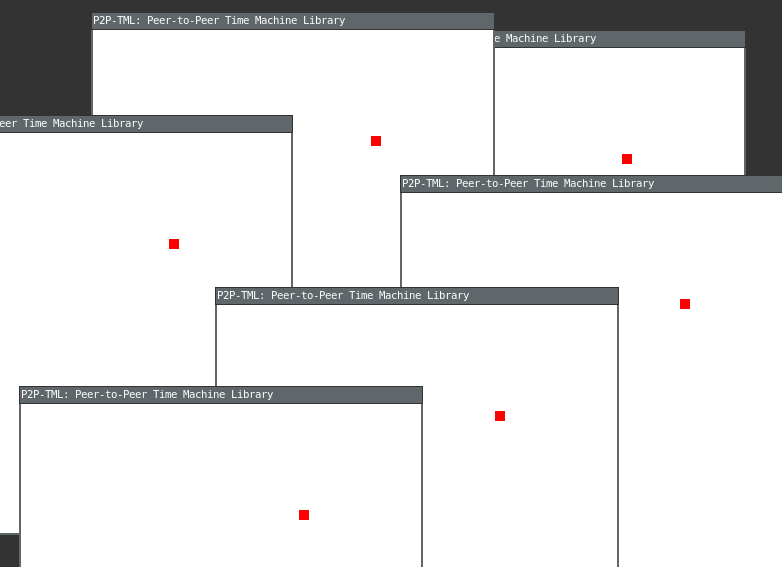
\includegraphics[width=\linewidth]{move}
    \caption[XXX] {
	A moving rectangle is controlled by peers connected indirectly.
	Users can press \code{↑ ↓ → ←} to change the direction of the
	rectangle or \code{SPACE} to pause the application.
	The inputs are applied simultaneously in all peers, as if they were
	mirrors of a single application.
        Video: \url{http://youtube.com/TODO}
        \label{fig.move}
    }
\end{figure}

- walk back-forth
- vector clocks
- dynamic net
- re-connect
- late join

We make some assumptions about the network, which are assigned externally to
the middleware:
%
\begin{itemize}
\item Peers have contiguous numeric unique identifiers.
\item Peers identifiers are assigned externally to the middleware.
\item Topology is dynamic, but also assigned externally

\end{itemize}
%
Except for the last item, we claim that the others can be solved externally,
without affecting the middleware.
For instance,
- orthogonal and would not affect the other algorithms in the middleware

, which we claim that could be
solved further:
- peers have unique identifiers
- ids are outside
- topology, dynamic but outside
- fixed maximum nodes
- fixed latency
We claim that Use external protocols
For instance, latency is only a constant, no problem being a variable

- non-malicious nodes

\section{Application}
\label{sec.app}

\section{Evaluation}
\label{sec.eval}

\section{Conclusion}
\label{sec.conclusion}

\bibliographystyle{IEEEtran}
\bibliography{tpd-22}

\begin{comment}
\begin{IEEEbiography}[{
\includegraphics[width=1in,height=1.25in,clip,keepaspectratio]{chico}}]{Francisco Sant'Anna}
received his PhD degree in Computer Science from PUC-Rio, Brazil in
2013.
In 2016, he joined the Faculty of Computer Science at the Rio de Janeiro State
University, Brazil.
His research interests include Programming Languages and Concurrent \&
Distributed Systems.
\end{IEEEbiography}
\end{comment}

\end{document}
